%%%%%%%%%%%%%%%%%%%%%%%%%%%%%%%%%%%%%%%%%
% Beamer Presentation
% LaTeX Template
% Version 1.0 (10/11/12)
%
% This template has been downloaded from:
% http://www.LaTeXTemplates.com
%
% License:
% CC BY-NC-SA 3.0 (http://creativecommons.org/licenses/by-nc-sa/3.0/)
%
%%%%%%%%%%%%%%%%%%%%%%%%%%%%%%%%%%%%%%%%%

%----------------------------------------------------------------------------------------
%	PACKAGES AND THEMES
%----------------------------------------------------------------------------------------

\documentclass[UTF8,aspectratio=169,14pt]{ctexbeamer}

\usepackage{hyperref}
\hypersetup{
	colorlinks=true,
	linkcolor=red,
	anchorcolor=blue,
	citecolor=green
}

\mode<presentation> {
	
	% The Beamer class comes with a number of default slide themes
	% which change the colors and layouts of slides. Below this is a list
	% of all the themes, uncomment each in turn to see what they look like.
	
	%\usetheme{default}
	%\usetheme{AnnArbor}
	%\usetheme{Antibes}
	%\usetheme{Bergen}
	%\usetheme{Berkeley}
	%\usetheme{Berlin}
	%\usetheme{Boadilla}
	%\usetheme{CambridgeUS}
	%\usetheme{Copenhagen}
	%\usetheme{Darmstadt}
	%\usetheme{Dresden}
	%\usetheme{Frankfurt}
	%\usetheme{Goettingen}
	%\usetheme{Hannover}
	%\usetheme{Ilmenau}
	%\usetheme{JuanLesPins}
	%\usetheme{Luebeck}
	\usetheme{Madrid}
	%\usetheme{Malmoe}
	%\usetheme{Marburg}
	%\usetheme{Montpellier}
	%\usetheme{PaloAlto}
	%\usetheme{Pittsburgh}
	%\usetheme{Rochester}
	%\usetheme{Singapore}
	%\usetheme{Szeged}
	%\usetheme{Warsaw}
	
	% As well as themes, the Beamer class has a number of color themes
	% for any slide theme. Uncomment each of these in turn to see how it
	% changes the colors of your current slide theme.
	
	%\usecolortheme{albatross}
	%\usecolortheme{beaver}
	%\usecolortheme{beetle}
	%\usecolortheme{crane}
	%\usecolortheme{dolphin}
	%\usecolortheme{dove}
	%\usecolortheme{fly}
	%\usecolortheme{lily}
	%\usecolortheme{orchid}
	%\usecolortheme{rose}
	%\usecolortheme{seagull}
	%\usecolortheme{seahorse}
	%\usecolortheme{whale}
	%\usecolortheme{wolverine}
	
	%\setbeamertemplate{footline} % To remove the footer line in all slides uncomment this line
	%\setbeamertemplate{footline}[page number] % To replace the footer line in all slides with a simple slide count uncomment this line
	
	%\setbeamertemplate{navigation symbols}{} % To remove the navigation symbols from the bottom of all slides uncomment this line
}

\usepackage{graphicx} % Allows including images
\graphicspath{{./figs/}}
\usepackage{booktabs} % Allows the use of \toprule, \midrule and \bottomrule in tables
\usepackage{longtable}
\usepackage{listings}
\usepackage{xcolor}
\lstset{numbers=left, %设置行号位置
	numberstyle=\tiny, %设置行号大小
	keywordstyle=\color{blue}, %设置关键字颜色
	commentstyle=\color[cmyk]{1,0,1,0}, %设置注释颜色
	frame=single, %设置边框格式
	escapeinside=``, %逃逸字符(1左面的键),用于显示中文
	%breaklines, %自动折行
	extendedchars=false, %解决代码跨页时,章节标题,页眉等汉字不显示的问题
	xleftmargin=2em,xrightmargin=2em, aboveskip=1em, %设置边距
	tabsize=4, %设置tab空格数
	showspaces=false %不显示空格
}
% Fonts
% \usepackage{libertine}
% \setmonofont{Courier}
\setCJKsansfont[ItalicFont=Noto Serif CJK SC Black, BoldFont=Noto Sans CJK SC Black]{Noto Sans CJK SC}


%----------------------------------------------------------------------------------------
% TITLE PAGE
%----------------------------------------------------------------------------------------

\title[第19讲]{第十九讲 :I/O子系统} % The short title appears at the bottom of every slide, the full title is only on the title page
\subtitle{第3节:磁盘子系统}
\author{向勇、陈渝} % Your name
\institute[清华大学] % Your institution as it will appear on the bottom of every slide, may be shorthand to save space
{
  清华大学计算机系 \\ % Your institution for the title page
  \medskip
  \textit{xyong,yuchen@tsinghua.edu.cn} % Your email address
}
\date{\today} % Date, can be changed to a custom date

\begin{document}

\begin{frame}
\titlepage % Print the title page as the first slide
\end{frame}

%----------------------------------------------
\begin{frame}
\frametitle{提纲} % Table of contents slide, comment this block out to remove it
\tableofcontents % Throughout your presentation, if you choose to use \section{} and \subsection{} commands, these will automatically be printed on this slide as an overview of your presentation

%% itemize
Ref:
    \begin{itemize}
        \item \href{http://osq.cs.berkeley.edu/public/JFoster-Drivers.ppt}{Linux Device Drivers Overview}
        \item \href{http://ermak.cs.nstu.ru/understanding.linux.kernel.pdf}{Understanding the Linux Kernel}
    \end{itemize}

\end{frame}
%----------------------------------------------
%%  PRESENTATION SLIDES
%----------------------------------------------
\section{第3节:磁盘子系统} % Sections can be created in order to organize your presentation into discrete blocks, all sections and subsections are automatically printed in the table of contents as an overview of the talk
%----------------------------------------------
%\subsection{Linux I/O Architecture} % A subsection can be created just before a set of slides with a common theme to further break down your presentation into chunks
%----------------------------------------------
\begin{frame}[fragile]
    \frametitle{磁盘概述}
%    \framesubtitle{xxxx}
%% figure
    磁盘工作机制和性能参数
    \begin{figure}
    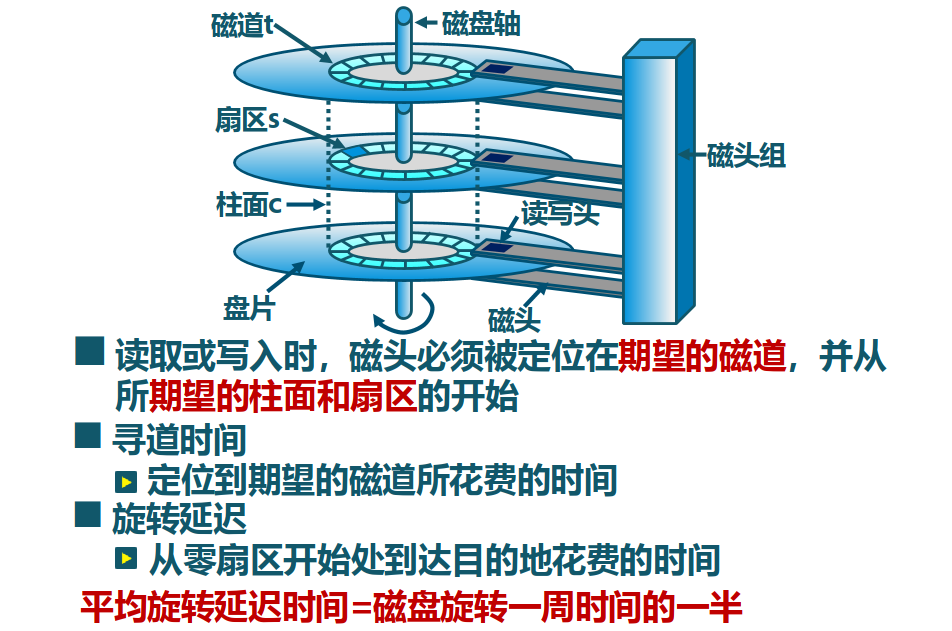
\includegraphics[width=0.57\linewidth]{figs/disk.png}
  %  \caption{xxxx}
    \end{figure}
\end{frame}

%----------------------------------------------
\begin{frame}[fragile]
    \frametitle{磁盘概述}
    %    \framesubtitle{xxxx}
    %% figure
    磁盘I/O传输时间
    \begin{figure}
        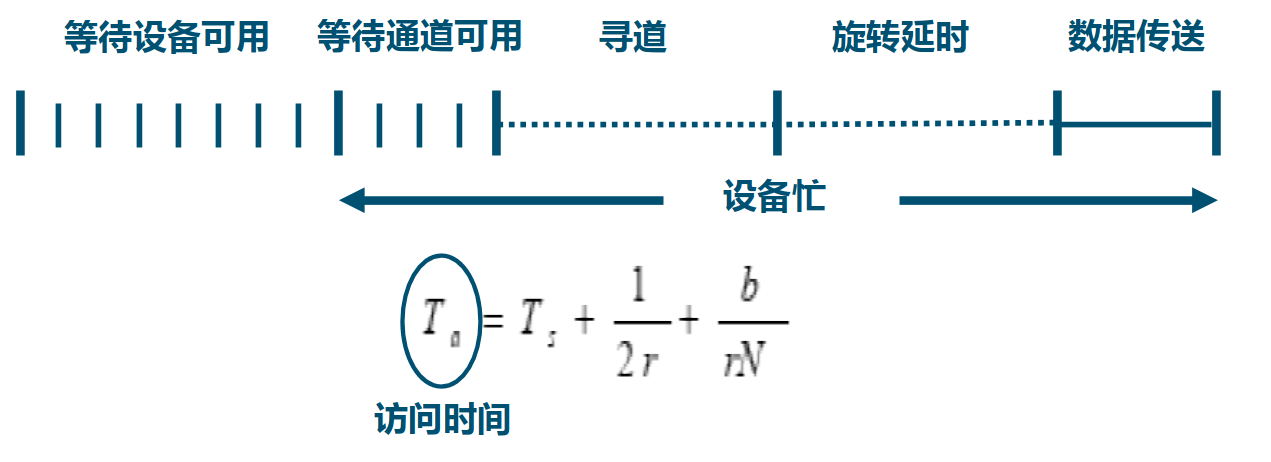
\includegraphics[width=0.8\linewidth]{figs/disk-time1.png}
        %  \caption{xxxx}
    \end{figure}
\end{frame}

%----------------------------------------------
\begin{frame}[fragile]
    \frametitle{磁盘概述}
    %    \framesubtitle{xxxx}
    %% figure
    磁盘I/O传输时间
    \begin{figure}
        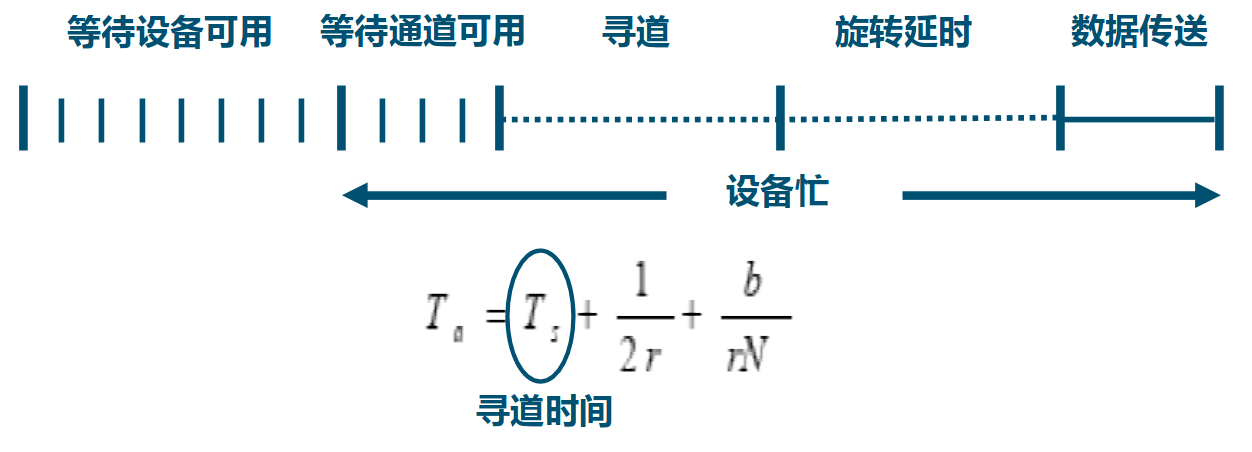
\includegraphics[width=0.8\linewidth]{figs/disk-time2.png}
        %  \caption{xxxx}
    \end{figure}
\end{frame}

%----------------------------------------------
\begin{frame}[fragile]
    \frametitle{磁盘概述}
    %    \framesubtitle{xxxx}
    %% figure
    磁盘I/O传输时间
    \begin{figure}
        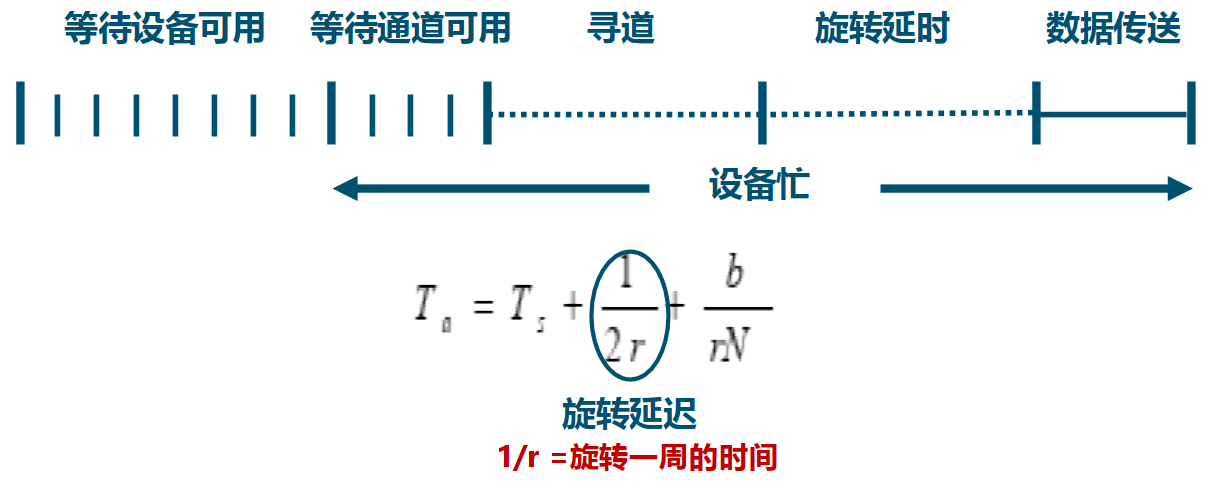
\includegraphics[width=0.8\linewidth]{figs/disk-time3.png}
        %  \caption{xxxx}
    \end{figure}
\end{frame}
%----------------------------------------------

%----------------------------------------------
\begin{frame}[fragile]
    \frametitle{磁盘概述}
    %    \framesubtitle{xxxx}
    %% figure
    磁盘I/O传输时间
    \begin{figure}
        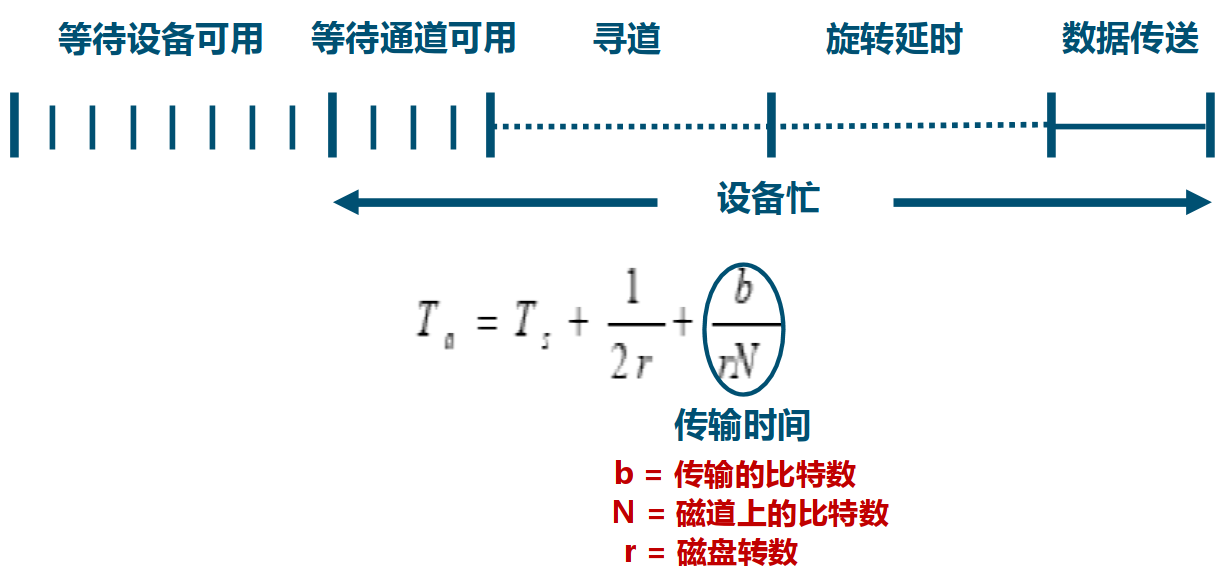
\includegraphics[width=0.8\linewidth]{figs/disk-time4.png}
        %  \caption{xxxx}
    \end{figure}
\end{frame}
%----------------------------------------------

\subsection{磁盘调度算法} % A subsection can be created just before a set of slides with a common theme to further break down your presentation into chunks
%----------------------------------------------
\begin{frame}[fragile]
    \frametitle{磁盘调度算法}
   通过优化磁盘访问请求顺序来提高磁盘访问性能
    \begin{itemize}
        \item 寻道时间是磁盘访问最耗时的部分
        \item 同时会有多个在同一磁盘上的I/O请求
        \item 随机处理磁盘访问请求的性能表现很差

    \end{itemize}
\end{frame}
%----------------------------------------------

%----------------------------------------------
\begin{frame}[fragile]
    \frametitle{磁盘调度算法}
    先进先出(FIFO)算法
    \begin{itemize}
        \item 按顺序处理请求
        \item 公平对待所有进程
        \item 在有很多进程的情况下,接近随机调度的性能
    \end{itemize}
\end{frame}

%----------------------------------------------
\begin{frame}[fragile]
    \frametitle{磁盘调度算法}
    先进先出(FIFO)算法
%    \begin{itemize}
%        \item 按顺序处理请求
%        \item 公平对待所有进程
%        \item 在有很多进程的情况下,接近随机调度的性能
%        \begin{itemize}
%            \item Locking, Interrupt time, resource allocation
%        \end{itemize}
%    \end{itemize}
    \begin{figure}
    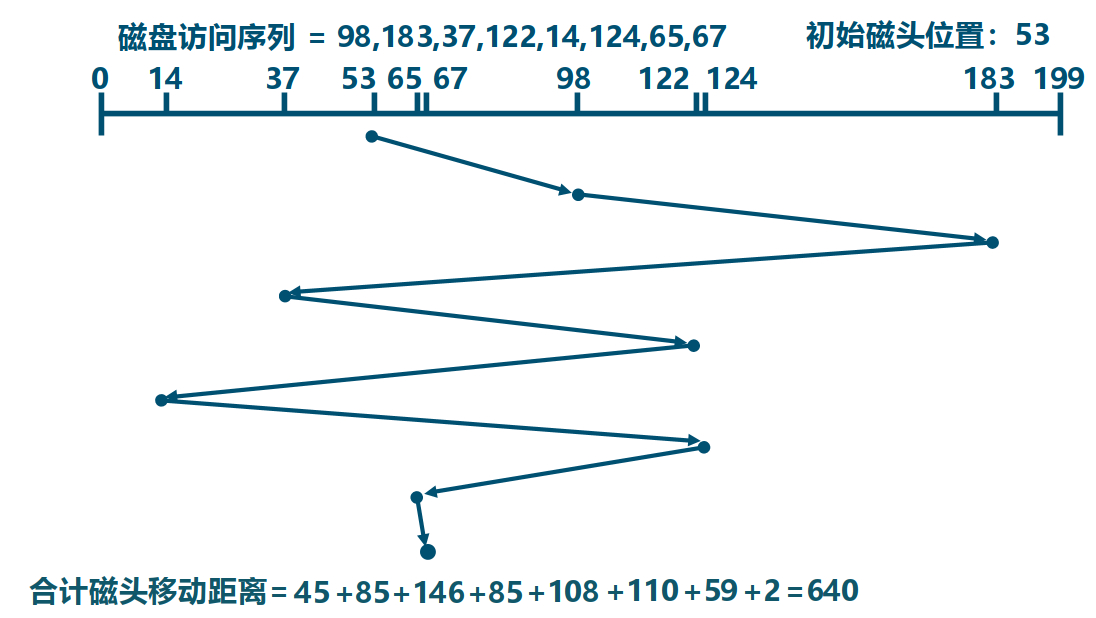
\includegraphics[width=0.7\linewidth]{figs/disk-fifo.png}
    %  \caption{xxxx}
\end{figure}
\end{frame}

%----------------------------------------------
\begin{frame}[fragile]
    \frametitle{磁盘调度算法}
    最短服务时间优先(SSTF)
    \begin{itemize}
        \item 选择从磁臂当前位置需要移动最少的I/O请求
        \item 总是选择最短寻道时间
    \end{itemize}
    \begin{figure}
    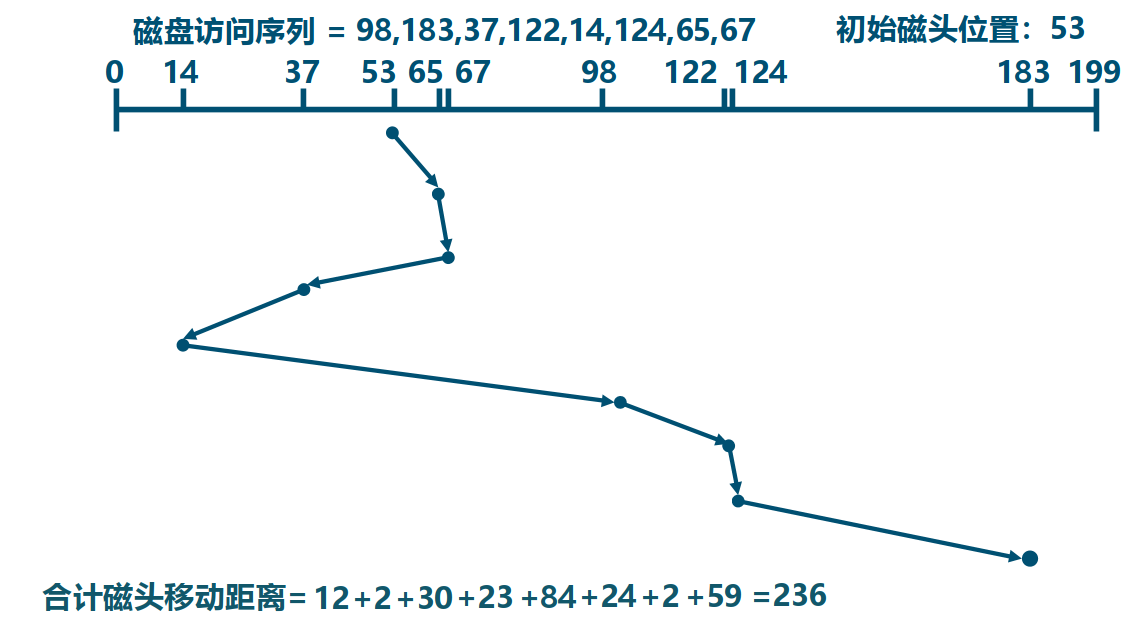
\includegraphics[width=0.65\linewidth]{figs/disk-sstf.png}
    %  \caption{xxxx}
    \end{figure}
\end{frame}

%----------------------------------------------
\begin{frame}[fragile]
    \frametitle{磁盘调度算法}
    扫描算法(SCAN)
    \begin{itemize}
        \item 磁臂在一个方向上移动,访问所有未完成的请求
        \item 直到磁臂到达该方向上最后的磁道,调换方向
        \item 也称为电梯算法(elevator algorithm)

    \end{itemize}
\end{frame}

%----------------------------------------------
\begin{frame}[fragile]
    \frametitle{磁盘调度算法}
    扫描算法(SCAN)
%    \begin{itemize}
%        \item 磁臂在一个方向上移动,访问所有未完成的请求
%        \item 直到磁臂到达该方向上最后的磁道,调换方向
%        \item 也称为电梯算法(elevator algorithm)
%        
%    \end{itemize}
\begin{figure}
    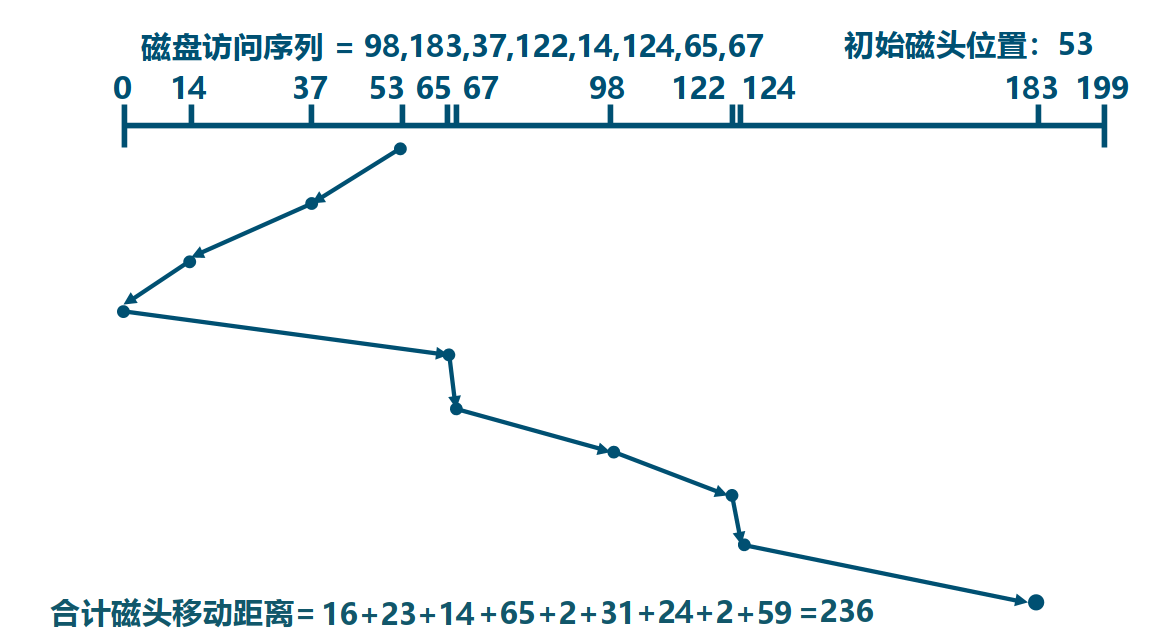
\includegraphics[width=0.7\linewidth]{figs/disk-scan.png}
%  \caption{xxxx}
\end{figure}
\end{frame}
%----------------------------------------------
\begin{frame}[fragile]
    \frametitle{磁盘调度算法}
    循环扫描算法(C-SCAN)
    \begin{itemize}
        \item 限制了仅在一个方向上扫描
        \item 当最后一个磁道也被访问过了后,磁臂返回到磁盘的另外一端再次进行
   \end{itemize}
    C-LOOK算法
   \begin{itemize}
       \item 磁臂先到达该方向上最后一个请求处,然后立即反转,而不是先到最后点路径上的所有请求

    \end{itemize}
\end{frame}
%----------------------------------------------
\begin{frame}[fragile]
    \frametitle{磁盘调度算法}
    N步扫描算法(N-step-SCAN)
    \begin{itemize}
        \item 磁头粘着(Arm Stickiness)现象
        \item SSTF、SCAN及CSCAN等算法中,可能出现磁头停留在某处不动的情况
    \end{itemize}
    N步扫描算法
    \begin{itemize}
        \item 将磁盘请求队列分成长度为N的子队列
        \item 按FIFO算法依次处理所有子队列
        \item 扫描算法处理每个队列        
    \end{itemize}
\end{frame}
%----------------------------------------------

%----------------------------------------------
\begin{frame}[fragile]
    \frametitle{磁盘调度算法}
    双队列扫描算法(FSCAN)
    \begin{itemize}
        \item FSCAN算法是N步扫描算法的简化
        \item FSCAN只将磁盘请求队列分成两个子队列
    \end{itemize}
    FSCAN算法
    \begin{itemize}
        \item 把磁盘I/O请求分成两个队列
        \item 交替使用扫描算法处理一个队列
        \item 新生成的磁盘I/O请求放入另一队列中
        \item 所有的新请求都将被推迟到下一次扫描时处理        
    \end{itemize}
\end{frame}
%----------------------------------------------
\end{document}
